\section{Bargaining over a rival's completion}
\label{sec:bargaining}

The 526 threads produce 920 responses: 113 acceptances, 394 counters and 413 rejections. Most bargaining is unsuccessful at the first offer. Only 32 of 524 acceptance-legal opening offers are accepted, and 81 settlements follow at least one counter. Table~\ref{tab:census} divides the offers by whose group the exchange would complete and by thread position.

\begin{table}[t]
\centering\small
\begin{tabular}{@{}lrrrrrrrr@{}}
\toprule
& \multicolumn{4}{c}{Opening offers} & \multicolumn{4}{c}{Later offers}\\
\cmidrule(lr){2-5}\cmidrule(lr){6-9}
Exchange completes a group for & $N$ & Acc. & Ctr. & Rej. & $N$ & Acc. & Ctr. & Rej.\\
\midrule
The author only & 187 & 3 & 46 & 138 \,(74\%) & 102 & 16 & 65 & 21 \,(21\%)\\
The recipient only & 51 & 2 & 18 & 31 \,(61\%) & 89 & 22 & 60 & 7 \,(8\%)\\
Both & 48 & 3 & 11 & 34 \,(71\%) & 33 & 7 & 24 & 2 \,(6\%)\\
Neither & 238 & 24 & 62 & 152 \,(64\%) & 170 & 36 & 107 & 27 \,(16\%)\\
\midrule
All & 524 & 32 & 137 & 355 & 394 & 81 & 256 & 57\\
\bottomrule
\end{tabular}
\caption{Responses to all 918 acceptance-legal offers. Completion is computed from the recipient's delivered holdings and includes mortgaged deeds. Cells differ in deeds, prices, players and game states; Appendix~\ref{app:bargaining} splits them by recipient.}
\label{tab:census}
\end{table}

\subsection{Refusal at the opening}

The clearest contrast is between opening offers that would complete only the author's group and opening offers that complete no group. The first are rejected in 74\% of cases and the second in 64\%, a difference of 9.9 points (Figure~\ref{fig:bargaining}a). The difference is positive in every seed block, at 15.0, 18.9, 5.8, 7.6 and 10.8 points, and stays between 8.7 and 11.3 points when any one block is left out. It is positive for each recipient that responds under the standard condition: 17.1 points for Sol, 5.1 for Gemini and 9.6 for Grok. Removing the 64 threads opened by a conflicting Grok call leaves 9.7 points. Removing every offer that Opus wrote or received raises it to 19.0 points, because Opus is the exception. As a recipient, Opus rejects 3 of 18 author-completing openings and 5 of 21 others.

\begin{figure}[t]
\centering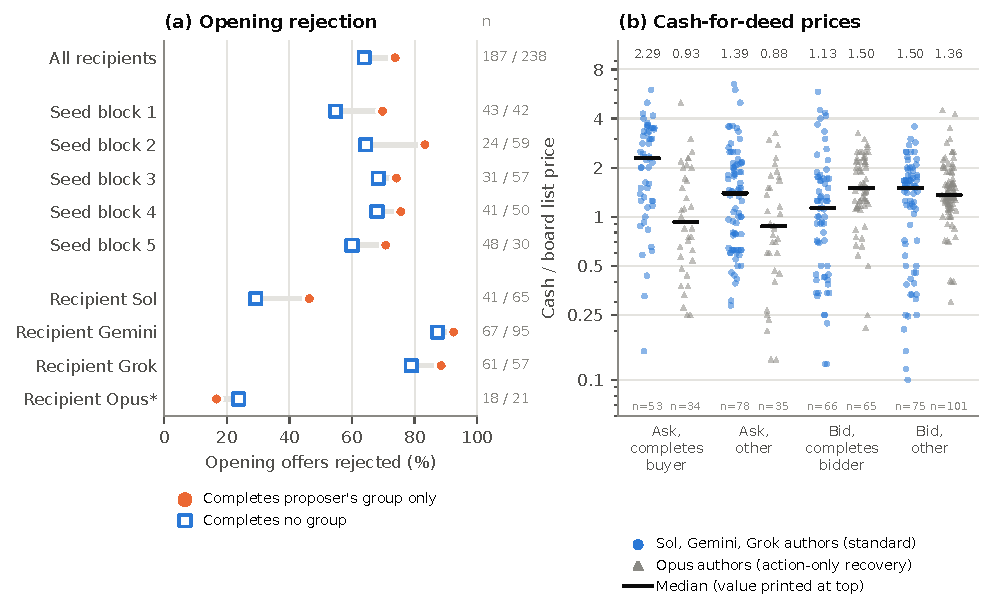
\includegraphics[width=\linewidth]{bargaining.pdf}
\caption{Defensive bargaining. (a) Share of opening offers rejected when the exchange would complete only the proposer's group (orange) or no group (blue), with offer counts. *Opus responds under action-only recovery in 162 of its 189 trade responses. (b) Cash-for-deed prices relative to board list price, for asks (written by the deed holder) and bids (written by the payer), separated by whether the deed would complete the buyer's group and by author condition. The pooled ask contrast holds in three of five seed blocks (Appendix~\ref{app:bargaining}).}
\label{fig:bargaining}
\end{figure}

The contrast does not reflect a general reluctance to trade with strong players. Opening rejection is 67\% when the author leads in asset value, 70\% when the recipient leads and 67\% when a third player leads. The response differs with whether this exchange completes the other party's group.

A sequence in G2 shows what this looks like from inside one negotiation.

\TranscriptTitle{g2}{One deed, two buyers, two prices}
Sol holds Marvin Gardens, the deed that would complete yellow for Opus, which owns the other two. Grok, which owns no yellow, bids \$200. That opening bid is itself one of Grok's conflicting calls: its content proposes to end the turn. Sol's counter prices the deed by what it could do in a third player's hands.
\TranscriptQuote{g2-d119-public}
\TranscriptQuote{g2-d119-note}
Grok answers with the same distinction between buyers.
\TranscriptQuote{g2-d120-public}
Sol rejects \$250.
\TranscriptQuote{g2-d121-public}
One turn later Opus bids \$325, and Sol asks the completing buyer for more.
\TranscriptQuote{g2-d124-price}
\TranscriptQuote{g2-d124-note}
The parties move to \$600 and \$450. Opus calls \$450 final while its own note records a ceiling of about \$475, and Sol keeps the deed.
\TranscriptQuote{g2-d128-keep}

\TranscriptFinding{Sol asked \$450 from the non-completing bidder and \$650, then \$600, from the completing one, and sold to neither. Its note's capacity arithmetic is wrong: \$520 buys three yellow houses at \$150, not nine. Twenty-four turns later the roles reverse. Opus, now holding \$17, trades its two yellows to Sol for two railroads and \$100, and Sol completes yellow. Opus is eliminated three turns later; Sol's yellows reach Gemini, the eventual winner, through Sol's own bankruptcy.}
\TranscriptReading{Both parties state that the same deed has different prices for different buyers, and Sol's ask follows that rule within one turn. The private note names a resale route to the completing player, so the seller is pricing a third party's option as well as the counterparty's. This is the identity-dependent pricing that the population contrasts look for. It is one seller and one deed, and the prices are asks, not settled values.}
\TranscriptSource{G2 d118--128 and d197--198. d119--121 are standard first attempts; d118 is a Grok conflict (content names \End). The quoted public messages appear in the counterparties' next requests.}

\subsection{Concessions rarely buy a completing deed}

Price concessions show the same asymmetry within threads. There are 199 offers in which an author keeps the same deeds as its previous offer and moves cash toward the recipient (Table~\ref{tab:concessions}). When the bundle would complete only the author's group, the recipient accepts 9 of 58 such concessions (16\%) and counters 39. When it completes nobody, the recipient accepts 24 of 86 (28\%). The median concession is \$60 and \$50 respectively. Without Opus as recipient the acceptance counts are 4 of 42 and 16 of 62. The ordering holds in four of the five seed blocks, but the blocks contain as few as three author-completing concessions, so we treat this as consistent with the opening contrast rather than as separate confirmation.

\begin{table}[t]
\centering\small
\begin{tabular}{@{}lrrrrr@{}}
\toprule
Exchange completes a group for & Concessions & Accepted & Countered & Rejected & Median concession\\
\midrule
The author only & 58 & 9 & 39 & 10 & \$60\\
The recipient only & 38 & 16 & 19 & 3 & \$50\\
Both & 17 & 6 & 11 & 0 & \$100\\
Neither & 86 & 24 & 49 & 13 & \$50\\
\bottomrule
\end{tabular}
\caption{Responses to within-thread cash concessions on an unchanged non-cash bundle.}
\label{tab:concessions}
\end{table}

Counters themselves are not specific to completion. Among counters to offers that request at least one deed, 79 of 111 to author-completing offers and 81 of 110 to non-completing offers return the same deeds and ask for more cash. Repricing an unchanged bundle is the agents' ordinary way to disagree. What differs is how often a better price ends the disagreement.

\subsection{Asking prices rise, bids do not}

If holders treat a completing deed as worth more to its buyer, their asks should rise when the buyer would complete a group. Pooled, they do. The median ask for a deed that would complete the buyer's group is 1.63 times list (87 asks), against 1.08 (113 asks) otherwise (Figure~\ref{fig:bargaining}b). Among the three standard-condition systems the medians are 2.29 and 1.39. Sol asks 2.32 against 1.80, and Grok 2.00 against 1.05. The ordering survives a split by whether the deed is mortgaged for Sol, Grok and Opus alike.

The pattern is weaker than the response contrast. It holds in only three of the five seed blocks; in blocks 1 and 5 asks to completing buyers are lower. The cleanest test is one seller asking for the same deed from two kinds of buyer in the same game, and there are only seven such single-deed comparisons. The first ask to the completing buyer is higher in five, lower in one and equal in one. In only three of the seven (G2, G16 and G20) is every ask to the completing buyer above every ask to the other buyer, and the asks are up to 106 turns apart. Opus's asks barely move with completion (0.93 against 0.88).

Bids show no matching premium. Standard-condition bidders offer a median of 1.13 times list for deeds that would complete their own group and 1.50 for others. Sol bids more for completion (1.88 against 1.25), Grok much less (0.50 against 1.54), and Opus slightly more (1.50 against 1.36). Holders thus price a rival's completion more consistently than buyers price their own. The asymmetry leaves a gap that neither side's offers close, which fits the low acceptance of completing deals. It is not an estimate of a premium, because deeds, stages and states differ across cells.

\subsection{What refusals cite, and what moves responses}

The agents' explanations name the rival's gain. In 74 outright rejections of offers that would complete the recipient's own group, both LLM-assisted readers found a stated consequence for the rival in 61 records ($\kappa=0.79$; 4 disagreements). The rate is 34 of 36 when both parties would complete and 27 of 38 when only the recipient would. Both readers also found a stated concern with the recipient's own price, cash or liquidity in 41 records ($\kappa=0.78$). The coded refusals come mostly from Gemini (31) and Grok (31). Sol writes only four outright rejections of this kind, and Opus eight, all without a private note. Thirty-one of the 61 agreed rival codes come from two games, G1 and G15.

The most common rival consequence is that the counterparty could build at once. We can test whether responses follow that quantity. For opening offers that would complete only the author's group, rejection is 75\% (100 of 134) when the author would keep enough cash for a full first layer of houses, 76\% (32 of 42) when it could afford at least one house but not a layer, and 55\% (6 of 11) when it could not afford one house. Later offers show the same flat profile, at 20\%, 21\% and one of three. The recipients do not reject more as the rival's building cash grows. Their response follows the category, a rival completing a group, rather than the amount they cite. The amount may still matter in ways these cells cannot show, since prices and deeds also vary across them.

\TranscriptTitle{g15}{Refusing one's own monopoly three times}
At G15 turn 63, Sol has \$730 and Grok \$333. Each holds a deed the other needs. Sol proposes a swap that completes both groups.
\TranscriptQuote{fx-g15-offer}
Grok's note on its refusal is about what each side could build afterwards.
\TranscriptQuote{fx-g15-refusal-note}
Sol drops its cash request, adds Kentucky, and then makes a third offer that answers the objection directly.
\TranscriptQuote{fx-g15-sweetener}
\TranscriptQuote{fx-g15-final-refusal}
\TranscriptFinding{No trade settles. The proposed balances of \$830 and \$233 match the ledger, and one house on each green would cost \$600, as Grok's note says, although a single green house costs \$200. Eighteen turns later Grok is the first player eliminated. Its yellow and green blockers pass to Gemini, which wins; Sol never completes either group.}
\TranscriptReading{Grok refuses its own complete group because the swap would let Sol build first, and keeps refusing after Sol changes the cash balance to meet that objection. The final offer would leave Grok with more cash than Sol, yet the reply moves to a different reason, Sol's mortgage capacity. The refusal is anchored on the rival's completion rather than on the cash figure it first cited. Whether refusing was wise cannot be judged from the records; the later elimination happens on a different path.}
\TranscriptSource{G15 d168--175, standard first attempts. The public messages appear in the counterparties' next requests; balances come from the rebuilt offer ledger.}

\subsection{Who sells completing deeds}

Completing deeds still change hands, and the sellers are short of cash. There are 22 settled cash-for-deed sales in which the deed completes the buyer's group and 31 in which it completes nothing (Figure~\ref{fig:distress}). Before the sale, 14 of the 22 completing sellers held less than \$100, against 7 of the 31 others; the median seller held \$61 against \$276. Opus sells 11 of the 22 completing deeds. Without Opus sellers the counts are 6 of 11 against 4 of 22, so the association is not only an Opus effect. The prices differ by seller condition: low-cash standard sellers still received a median of 2.25 times list, while Opus's eight low-cash sales cleared at a median of 0.66 times list.

\begin{figure}[t]
\centering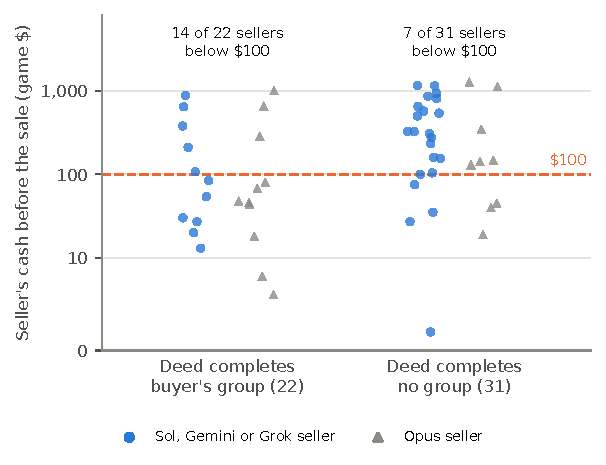
\includegraphics[width=0.66\linewidth]{distress.pdf}
\caption{Seller's cash immediately before each settled cash-for-deed sale, by whether the deed completed the buyer's group (symmetric log scale). Opus sellers are marked separately because Opus played under action-only recovery.}
\label{fig:distress}
\end{figure}

This population conditions on settlement, so it does not show that cash pressure causes sales. It shows which completing sales happened. Read with the refusals and the unanswered concessions, it suggests that holders give up a rival's completing deed mostly when they need the money, and that standard-condition sellers still charge for it.

Defensive bargaining can also be collective. In G20, a public appeal asks the whole table to deny a rival the cash it needs to build.

\TranscriptTitle{g20}{An appeal to withhold a rival's building cash}
Opus has just sold Illinois to Grok for \$500, completing Grok's reds and leaving it \$222. A red house costs \$150. Gemini addresses the table.
\TranscriptQuote{g20-coordination-appeal}
Grok's next private note records the appeal.
\TranscriptQuote{g20-recognition-note}
After building, Grok offers Vermont to Gemini for \$150, and Gemini declines.
\TranscriptQuote{g20-concrete-refusal}
\TranscriptFinding{Grok mortgages Vermont for \$50 instead. Sol had already recorded its own objection to funding Grok in a private note at d95. Opus later makes two cash offers for Grok's property, and neither settles. Gemini wins the game.}
\TranscriptReading{Gemini states the denial rule as a public appeal and follows it when tested. The appeal is a collective version of the defensive pattern. The records show one appeal, its author's compliance and one other player's prior agreement in private; Opus's later bids show that the norm was not adopted by everyone.}
\TranscriptSource{G20 d95--102 and d129--160. The appeal appears in Grok's d97 request; the quoted note is from Grok's selected attempt 1, after a malformed first attempt.}

\subsection{The Opus exception}

Opus departs from the defensive pattern at each step. As a recipient it rejects proposer-completing openings less often than other openings, it accepts 5 of 16 completing concessions, and its asks hardly change with completion. It also opens 240 of the 526 threads and bids above list for completing deeds. Opus played most decisions without a private note and without a corrective retry. These records cannot separate the model from that condition, and we do not attribute its behaviour to either. What they do show is that one of the four players was a ready trading partner, and that 8 of the 14 distressed completing sales came from it. The other agents' defensive bargaining took place in a market that contained this partner.
